% % % % % % % % % % % % % % % % % % % % % % % % % % % % % % % % % % % % % % % %
% IEEE Style - Double columns, 11pt font, letterpaper
\documentclass[journal, twocolumn, final,11pt,letterpaper]{IEEEtran}	

% Include Latex Packages
\usepackage{etex}	% This package enables the use of many packages

% % Page styles
\usepackage{setspace}	% line spacing package
\doublespacing			% use double spacing
%\linespread{1.6}		% Use linespread to fine tune line spacing, not recommended


% % Figures
\usepackage{float}		% improves interface for floating objects
\usepackage{subfig}		% enables subfloat
\usepackage{graphicx}	% more image type support
\usepackage{circuitikz}
\usepackage{epstopdf}	% automatically convert included eps files to pdf
\usepackage{tikz}
%\usepackage{listings}
\usepackage{color}
\definecolor{dkgreen}{rgb}{0,0.6,0}
\definecolor{gray}{rgb}{0.5,0.5,0.5}
\definecolor{mauve}{rgb}{0.58,0,0.82}

\lstset{frame=tb,
	language=Verilog,
	aboveskip=3mm,
	belowskip=3mm,
	showstringspaces=false,
	columns=flexible,
	basicstyle={\small\ttfamily},
	numbers=none,
	numberstyle=\tiny\color{gray},
	keywordstyle=\color{blue},
	commentstyle=\color{dkgreen},
	stringstyle=\color{mauve},
	breaklines=true,
	breakatwhitespace=true,
	tabsize=3
}
\usetikzlibrary{matrix,calc}
\usetikzlibrary{shapes}

\newcommand*{\circled}[2][red]{
	\tikz[baseline=(char.base)]{
		\node[shape=ellipse,inner sep=1pt,
		draw=#1,
		] (char) {#2};}
}

%isolated term
%#1 - Optional. Space between node and grouping line. Default=0
%#2 - node
%#3 - filling color
\newcommand{\implicantsol}[3][0]{
	\draw[rounded corners=3pt, fill=#3, opacity=0.3] ($(#2.north west)+(135:#1)$) rectangle ($(#2.south east)+(-45:#1)$);
}


%internal group
%#1 - Optional. Space between node and grouping line. Default=0
%#2 - top left node
%#3 - bottom right node
%#4 - filling color
\newcommand{\implicant}[4][0]{
	\draw[rounded corners=3pt, fill=#4, opacity=0.3] ($(#2.north west)+(135:#1)$) rectangle ($(#3.south east)+(-45:#1)$);
}

%group lateral borders
%#1 - Optional. Space between node and grouping line. Default=0
%#2 - top left node
%#3 - bottom right node
%#4 - filling color
\newcommand{\implicantcostats}[4][0]{
	\draw[rounded corners=3pt, fill=#4, opacity=0.3] ($(rf.east |- #2.north)+(90:#1)$)-| ($(#2.east)+(0:#1)$) |- ($(rf.east |- #3.south)+(-90:#1)$);
	\draw[rounded corners=3pt, fill=#4, opacity=0.3] ($(cf.west |- #2.north)+(90:#1)$) -| ($(#3.west)+(180:#1)$) |- ($(cf.west |- #3.south)+(-90:#1)$);
}

%group top-bottom borders
%#1 - Optional. Space between node and grouping line. Default=0
%#2 - top left node
%#3 - bottom right node
%#4 - filling color
\newcommand{\implicantdaltbaix}[4][0]{
	\draw[rounded corners=3pt, fill=#4, opacity=0.3] ($(cf.south -| #2.west)+(180:#1)$) |- ($(#2.south)+(-90:#1)$) -| ($(cf.south -| #3.east)+(0:#1)$);
	\draw[rounded corners=3pt, fill=#4, opacity=0.3] ($(rf.north -| #2.west)+(180:#1)$) |- ($(#3.north)+(90:#1)$) -| ($(rf.north -| #3.east)+(0:#1)$);
}

%group corners
%#1 - Optional. Space between node and grouping line. Default=0
%#2 - filling color
\newcommand{\implicantcantons}[2][0]{
	\draw[rounded corners=3pt, opacity=.3] ($(rf.east |- 0.south)+(-90:#1)$) -| ($(0.east |- cf.south)+(0:#1)$);
	\draw[rounded corners=3pt, opacity=.3] ($(rf.east |- 8.north)+(90:#1)$) -| ($(8.east |- rf.north)+(0:#1)$);
	\draw[rounded corners=3pt, opacity=.3] ($(cf.west |- 2.south)+(-90:#1)$) -| ($(2.west |- cf.south)+(180:#1)$);
	\draw[rounded corners=3pt, opacity=.3] ($(cf.west |- 10.north)+(90:#1)$) -| ($(10.west |- rf.north)+(180:#1)$);
	\fill[rounded corners=3pt, fill=#2, opacity=.3] ($(rf.east |- 0.south)+(-90:#1)$) -|  ($(0.east |- cf.south)+(0:#1)$) [sharp corners] ($(rf.east |- 0.south)+(-90:#1)$) |-  ($(0.east |- cf.south)+(0:#1)$) ;
	\fill[rounded corners=3pt, fill=#2, opacity=.3] ($(rf.east |- 8.north)+(90:#1)$) -| ($(8.east |- rf.north)+(0:#1)$) [sharp corners] ($(rf.east |- 8.north)+(90:#1)$) |- ($(8.east |- rf.north)+(0:#1)$) ;
	\fill[rounded corners=3pt, fill=#2, opacity=.3] ($(cf.west |- 2.south)+(-90:#1)$) -| ($(2.west |- cf.south)+(180:#1)$) [sharp corners]($(cf.west |- 2.south)+(-90:#1)$) |- ($(2.west |- cf.south)+(180:#1)$) ;
	\fill[rounded corners=3pt, fill=#2, opacity=.3] ($(cf.west |- 10.north)+(90:#1)$) -| ($(10.west |- rf.north)+(180:#1)$) [sharp corners] ($(cf.west |- 10.north)+(90:#1)$) |- ($(10.west |- rf.north)+(180:#1)$) ;
}

%Empty Karnaugh map 4x4
\newenvironment{Karnaugh}%
{
	\begin{tikzpicture}[baseline=(current bounding box.north),scale=0.8]
	\draw (0,0) grid (4,4);
	\draw (0,4) -- node [pos=0.9,above right,anchor=south west] {C1C0} node [pos=0.9,below left,anchor=north east] {EQ} ++(135:1);
	%
	\matrix (mapa) [matrix of nodes,
	column sep={0.8cm,between origins},
	row sep={0.8cm,between origins},
	every node/.style={minimum size=0.3mm},
	anchor=8.center,
	ampersand replacement=\&] at (0.5,0.5)
	{
		\& |(c00)| 00         \& |(c01)| 01         \& |(c11)| 11         \& |(c10)| 10         \& |(cf)| \phantom{00} \\
		|(r00)| 00             \& |(0)|  \phantom{0} \& |(1)|  \phantom{0} \& |(3)|  \phantom{0} \& |(2)|  \phantom{0} \&                     \\
		|(r01)| 01             \& |(4)|  \phantom{0} \& |(5)|  \phantom{0} \& |(7)|  \phantom{0} \& |(6)|  \phantom{0} \&                     \\
		|(r11)| 11             \& |(12)| \phantom{0} \& |(13)| \phantom{0} \& |(15)| \phantom{0} \& |(14)| \phantom{0} \&                     \\
		|(r10)| 10             \& |(8)|  \phantom{0} \& |(9)|  \phantom{0} \& |(11)| \phantom{0} \& |(10)| \phantom{0} \&                     \\
		|(rf) | \phantom{00}   \&                    \&                    \&                    \&                    \&                     \\
	};
}%
{
	\end{tikzpicture}
}

%Empty Karnaugh map 2x4
\newenvironment{Karnaughvuit}%
{
	\begin{tikzpicture}[baseline=(current bounding box.north),scale=0.8]
	\draw (0,0) grid (4,2);
	\draw (0,2) -- node [pos=0.7,above right,anchor=south west] {LA/LB} node [pos=0.6,below left,anchor=north east] {S} ++(120:1);
	%
	\matrix (mapa) [matrix of nodes,
	column sep={0.8cm,between origins},
	row sep={0.8cm,between origins},
	every node/.style={minimum size=0.3mm},
	anchor=4.center,
	ampersand replacement=\&] at (0.5,0.5)
	{
		\& |(c00)| 00         \& |(c01)| 01         \& |(c11)| 11         \& |(c10)| 10         \& |(cf)| \phantom{00} \\
		|(r00)| 0             \& |(0)|  \phantom{0} \& |(1)|  \phantom{0} \& |(3)|  \phantom{0} \& |(2)|  \phantom{0} \&                     \\
		|(r01)| 1             \& |(4)|  \phantom{0} \& |(5)|  \phantom{0} \& |(7)|  \phantom{0} \& |(6)|  \phantom{0} \&                     \\
		|(rf) | \phantom{00}  \&                    \&                    \&                    \&                    \&                     \\
	};
}%
{
	\end{tikzpicture}
}

%Empty Karnaugh map 2x2
\newenvironment{Karnaughquatre}%
{
	\begin{tikzpicture}[baseline=(current bounding box.north),scale=0.8]
	\draw (0,0) grid (2,2);
	\draw (0,2) -- node [pos=0.7,above right,anchor=south west] {b} node [pos=0.7,below left,anchor=north east] {a} ++(135:1);
	%
	\matrix (mapa) [matrix of nodes,
	column sep={0.8cm,between origins},
	row sep={0.8cm,between origins},
	every node/.style={minimum size=0.3mm},
	anchor=2.center,
	ampersand replacement=\&] at (0.5,0.5)
	{
		\& |(c00)| 0          \& |(c01)| 1  \\
		|(r00)| 0 \& |(0)|  \phantom{0} \& |(1)|  \phantom{0} \\
		|(r01)| 1 \& |(2)|  \phantom{0} \& |(3)|  \phantom{0} \\
	};
}%
{
	\end{tikzpicture}
}

%Defines 8 or 16 values (0,1,X)
\newcommand{\contingut}[1]{%
	\foreach \x [count=\xi from 0]  in {#1}
	\path (\xi) node {\x};
}

%Places 1 in listed positions
\newcommand{\minterms}[1]{%
	\foreach \x in {#1}
	\path (\x) node {1};
}

%Places 0 in listed positions
\newcommand{\maxterms}[1]{%
	\foreach \x in {#1}
	\path (\x) node {0};
}

%Places X in listed positions
\newcommand{\indeterminats}[1]{%
	\foreach \x in {#1}
	\path (\x) node {X};
}



% % Maths
\usepackage[cmex10]{amsmath}	% Maths
\usepackage{amsfonts,amssymb} 	% maths symbols

% % Tables
\usepackage{booktabs}  % professional-looking tables
\usepackage{multicol} %used for getting multicolumn without page-break
\usepackage{multirow}	% multi-row tables
\usepackage{array}		% define column format of a table

% % Others
\usepackage{caption}	%Customising captions in floating environments
%\usepackage{abstract}
\usepackage{cite}		% cite multiple
\usepackage{fixltx2e}	%added by pilawa, preventing figure* to get ahead of regular figures.
\usepackage{url}		% url display

% %
\hyphenation{op-tical net-works semi-conduc-tor}	% correct bad hyphenation here
\providecommand{\e}[1]{\ensuremath{\times 10^{#1}}}		% use use \e{2} for scientific number expression


% % Optional packages that might be useful
%\usepackage{epsf}		% eps fix
%\usepackage{verbatim}	% verbatim text are not interpreted by the compiler 
%\numberwithin{equation}{section}	% number equation according to section
%\usepackage{xfrac}		% slanted fraction
%\usepackage{pgfplots}	% plot graph
%\usepackage{tikz,pgfplots} % plot graph
%\usepackage{endnotes}	% endnotes


% Title of Document
\title{ECE385 Experiment \#2
	}
\author{
\IEEEauthorblockN{Eric Meyers, Ryan Helsdingen}\\
\IEEEauthorblockA{Section ABG; TAs: Ben Delay, Shuo Liu \\
February 3rd, 2016 \\
emeyer7, helsdin2\vspace{-10mm}}}
% % % % % % % % % % % % % % % % % % % % % % % % % % % % % % % % % % % % % % % 
\begin{document}
	
%SECTION : Formatting and Title
\maketitle
\singlespacing

%SECTION 1 - Introduction
\vspace{-20mm}
\section{Introduction}
\IEEEPARstart{T}{he} purpose of this lab is to create a synchronous storage unit consisting of two four-bit shift registers, plus some control logic, which will have four basic operations: \emph{load, read, write, and do nothing}. The idea behind creating a storage unit out of shift registers is to explore different implementations of RAM and to explore basic principles of storing and loading digital data. 

\vspace{-4mm}

%SECTION 2 - Description of Circuit
\section{Description of Circuit}
As stated above, the primary purpose of the circuit that was designed in this lab was to create a 4-by-2 bit storage unit out of shift registers and TTL chips. As with any storage unit, the operator must be able to specify whether they would like to "write" or "read" to/from the storage. Therefore, there must be a convention used to choose a specific address from the unit and read those contents into a buffer. \\

For this lab, the Storage Address Register (SAR) will contain the address being read, and the Storage Buffer Register (SBR) will contain the contents from the address specified by SAR. \\

Three switches were used on the I/O switchboard to achieve the read/write commands: STORE, FETCH, and LDSBR. Two switches were used for the data-in given by the user (DIN0, DIN1). Finally, two more switches were used so that the user can specify the SAR for reading (SAR0, SAR1), for a total of 7 switches used on the I/O switchboard. \\

The actual storage of data is implemented by using a universal shift register that is loading in one bit at a time through the serial-right input. This shift register is continuously shifting its contents, which are specified by the user. "Read" and "write" commands are accomplished by setting the FETCH or STORE signal high. \\

A STORE signal takes the contents specified by the SBR and moves it into the shift register to the appropriate location specified by the SAR.\\

LDSBR is used to store the data specified by the user from the DIN1 and DIN0 switches into the SBR. \\ 

A FETCH signal takes the contents in the address specified by the SAR and stores it into the SBR. \\

Because the bits are continuously shifting inside the shift register, some control logic must be added to select the proper address specified by the user in the SAR. In order to do that, a two-bit counter must be used along with a comparator to check to see if the proper address is being accessed inside the shift register. \\

The MUXs were used for selection logic on loading into the SBR register and determining the proper timing to load into the correct address as specified by the counter.

The following TTL chips were used:
\begin{itemize}
	\item 4-bit Binary Counter - SNLS169
	\item 4-bit Magnitude Comparator - DM74LS85
	\item (2) 4-bit Universal Shift Register - SN74LS193
	\item 4-to-1 MUX - DM54LS153	
	\item 2-to-1 MUX - DM54LS157
	\item Quad 2-Input NAND - DM54LS00
	\item Quad D-Latch - DM74LS75 \\
\end{itemize} 

These components were assembled on a protoboard and (as stated earlier) connected to a I/O switchboard which allows the operator to control the bits going in/out of the system. The protoboard was then connected to a function generator used to generate a 1 kHz 5 V peak-to-peak square-wave with +2.5V offset used for the clock in the components. \\


%SECTION 3 - Block Diagram
\section{Block Diagram}
Please refer to Figure \ref{fig:block-diagram} in "Section IX: Figures" of this document for the Block Diagram of the Storage Unit.  

%SECTION 4 - Design
\section{Design}
A truth table was created to determine the control logic on both the MUXs and the comparator. Please refer to Figure \ref{fig:truth-table-control} in "Section IX: Figures" of this document for the Control Logic Truth Table created during the prelab. \\

The team then created a Karnaugh-Map from this truth table to determine the proper minterms and the resulting logic function for each of the multiplexers. The K-Map for the 4-to-1 MUX selection logic is shown below. FETCH is represented by "F", LDSBR is represented by "L", and "CompareOUT" is represented by C.
 \begin{figure} [H]
 	\centering
	 \begin{Karnaughvuit}
	 	\minterms{0,1,2,4,5}
	 	\maxterms{6}
	 	\indeterminats{3, 7}
	 	\implicant{0}{5}{lightgray}
	 	\implicant{0}{2}{lightgray}
	\end{Karnaughvuit}
	\vspace{-5mm}
	\caption*{Selction Line 1 (S1)}
 \end{figure}
 \vspace{-5mm}
\begin{figure}[H]
	\centering
	\begin{Karnaughvuit} 
		\minterms{0,1,2,4,6}
		\maxterms{5}
		\indeterminats{3,7}
		\implicant{0}{2}{lightgray}
		\implicantcostats{0}{6}{lightgray}
	\end{Karnaughvuit}
	\vspace{-5mm}
	\caption*{Selection Line 0 (S0)}
\end{figure}

This gives us SOP function as follows:
\begin{center}
S1 = $\lnot$ C $\lor$ $\lnot$ L \\
S0 = $\lnot$ C $\lor$ $\lnot$ F
\end{center}
These logic functions were then constructed into a AND-OR circuit, then converted into a NAND-NAND circuit using deMorgan's Laws.\\ 

The selection logic for the 2-to-1 MUX was much less complex than the logic for the 4-to-1 MUX and simply was a direct line to a NAND of the comparator and the STORE signal. This is so that it can store the proper signal when the correct address is reached in the counter.
 
%SECTION 5 - Component Layout Sheet
\section{Component Layout Sheet}
Please refer to Figure \ref{fig:component-layout} in "Section IX: Figures" of this document for the Component Layout Diagram created during the prelab.

%SECTION 6 - Circuit/Logic Diagrams
\section{Circuit/Logic Diagrams}
Please refer to Figure \ref{fig:logic-diagram} in "Section IX: Figures" of this document for the Logic Diagram of the Storage Unit.  

%SECTION 7 - Documentation
\vspace{-2mm}
\section{Documentation from Experiment}
The documentation required from the lab is expalined throughout this document as needed. Please refer to those sections as necessary. 

%SECTION 8 - Conclusion
\section{Conclusion}
Overall, the team managed to design and construct a synchronous 4-by-2 bit storage unit from shift registers, however some minor setbacks occured with the implementation of our circuit.\\ 

The circuit was constructed prior to lab and during the testing phase, the team encountered a problem in the logic. The storage unit would allow the user to store into the SBR using LDSBR and the DIN switches perfectly and consistently. The storage unit would also allow the user to write these values (in the SBR) into the shift-register using the LOAD switch. However, if the user loaded words into the shift-register in a particular order, and attempted to fetch one of those values, using the FETCH switch, the values read into SBR would be incorrect. Specifically, instead of a solid color indicating high/low on the LED, the SBR would blink the "correct" value every fourth clock-cycle. \\

The team narrowed this down to a problem in the logic with both the LDSBR and FETCH switch. This is because when both the FETCH switch and the LDSBR switch were turned on, the system would function properly and output the correct values to the LED. The team tried to further examine the error and attempted to deconstruct the logic to correct the circuit. \\

When FETCH is on and LDSBR is off, the improper values were being fetched from the shift register during three clock cycles, and when FETCH is on and LDSBR is on, the SBR was being loaded with the proper value during one clock cycle and was doing nothing on the other three clock cycles, which is the intended functionality.\\

The team then constructed truth tables of the improper logic (shown in the below table), and it was concluded that a single bit was being flipped, which led to the intended functionality during when LDSBR and FETCH were both on.

\begin{center}
	\begin{tabular}{lll|ll}
		C & F & L & S1 & S0 \\ \hline
		0 & 0 & 0 & 1 & 1\\
		0 & 0 & 1 & 1 & 1 \\
		0 & 1 & 0 & \hspace{-2mm}\circled[red]0 & 1 \\
		... & ... & ...& ... & ... \\
		
		
	\end{tabular}
\end{center}

The team then realized that the NAND gates were improperly wired in the circuit that was constructed. This is what led to the single bit being flipped in the table above. \\

The team unfortunately ran out of time attempting to fix the error however, received almost-full credit on the demo. \\

The prelab circuit was the same design as the final circuit, so there are no changes to document. However, due to wiring inconsistencies.

Some other possible causes of error might be synchronization issues. The function generator was daisy-chained to each chip which might have caused an issue in the timing of the rising edge of the clock cycle. \\

\newpage
\onecolumn
%SECTION 9: Figures
\section{Figures}
\begin{figure}[h]
	\centering
	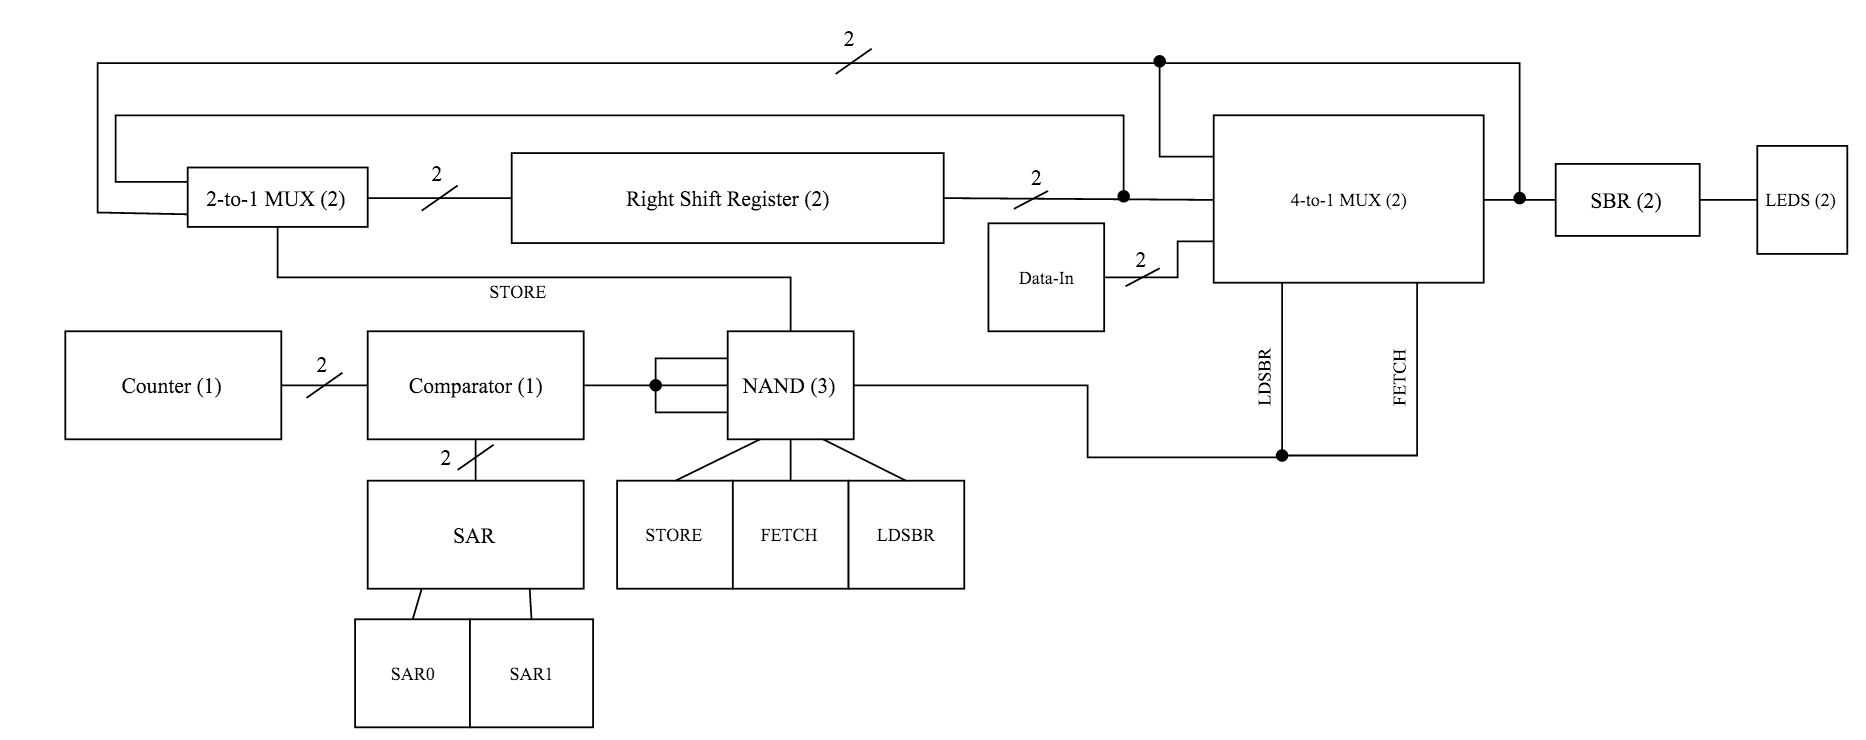
\includegraphics[scale=0.55]{Block_Diagram.png}
	\caption{Block Diagram from Pre-Lab}
	\label{fig:block-diagram}
\end{figure}

\begin{figure}[h]
	\centering
	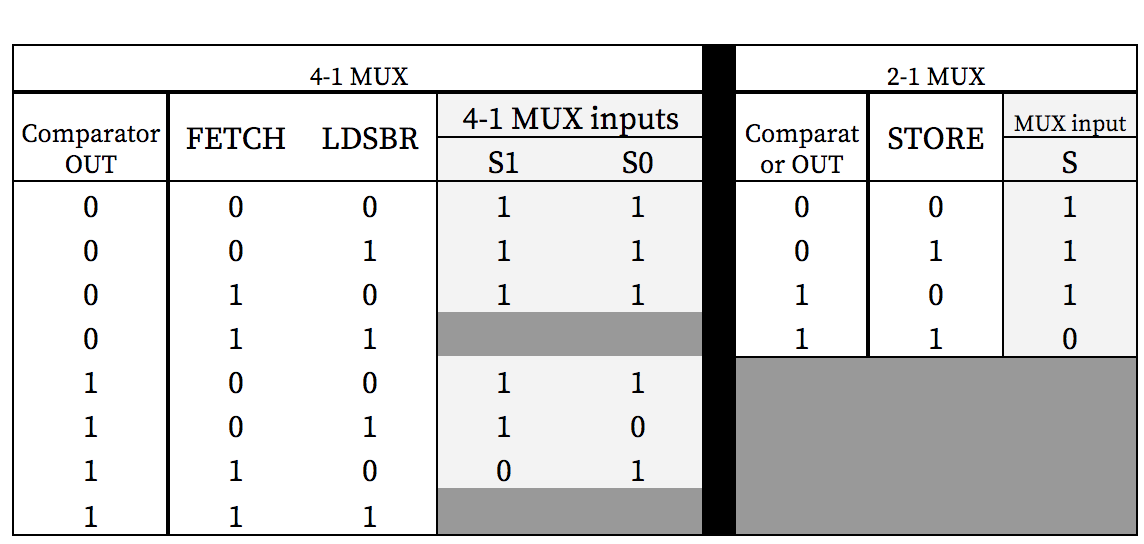
\includegraphics[scale=0.75]{Control_Logic_Truth_Table.png}
	\caption{Control Logic Truth Table from Pre-Lab}
	\label{fig:truth-table-control}
\end{figure}

\begin{figure}[h]
	\centering
	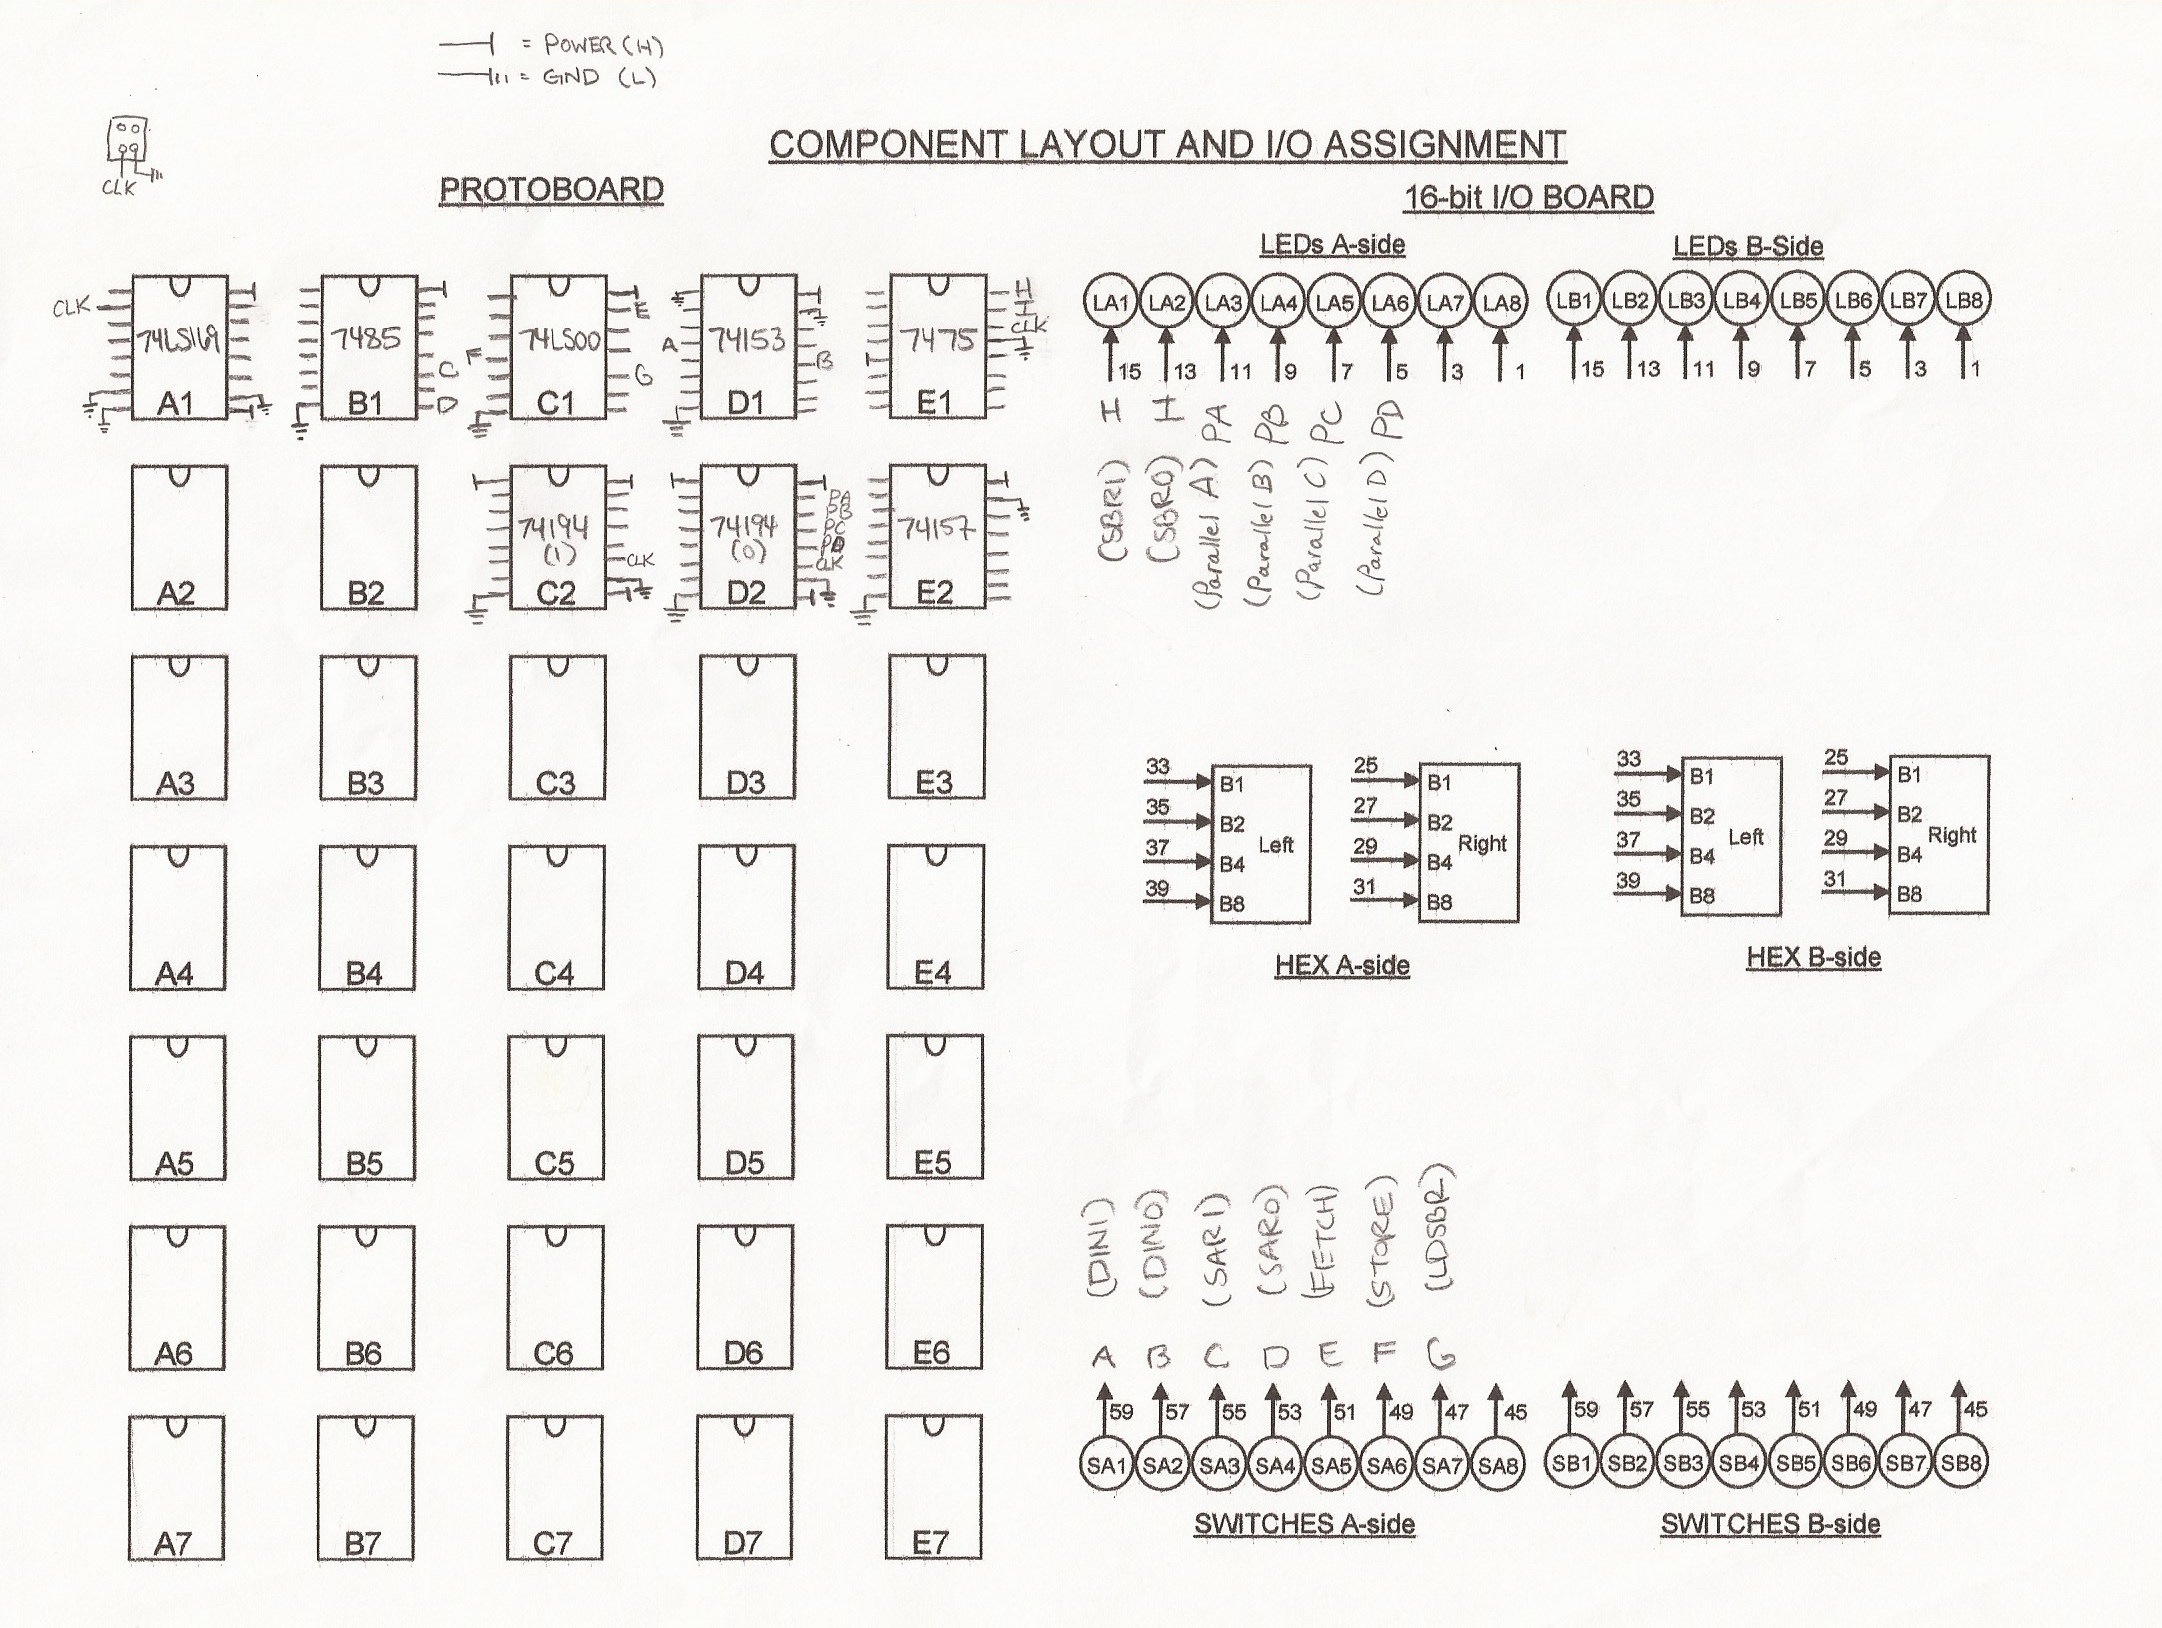
\includegraphics[scale=0.19]{Component_Layout.jpeg}
	\caption{Component Layout for Storage Unit}
	\label{fig:component-layout}
\end{figure}

\begin{figure}[h]
	\centering
	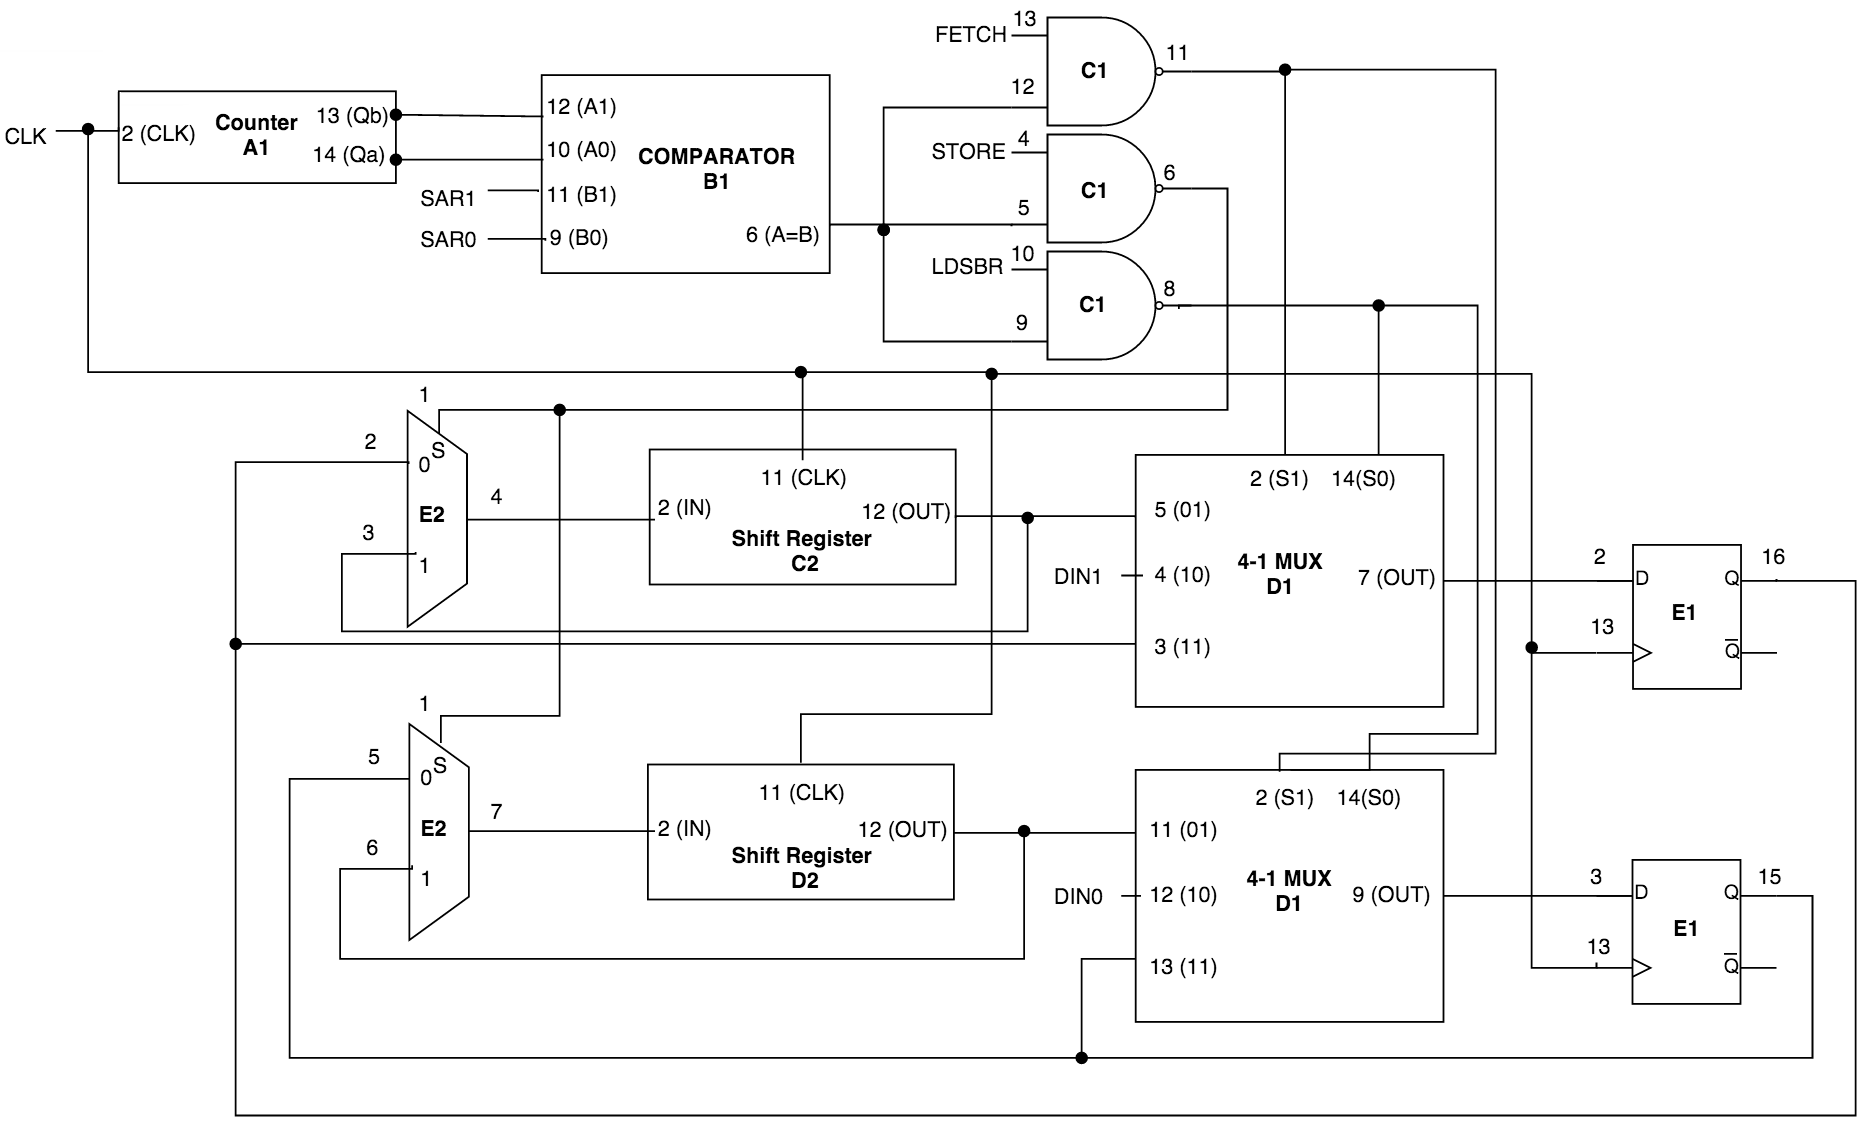
\includegraphics[scale=0.43]{Logic_Diagram.png}
	\caption{Logic Diagram from Pre-Lab}
	\label{fig:logic-diagram}
\end{figure}

\begin{figure}[h]
	\centering
	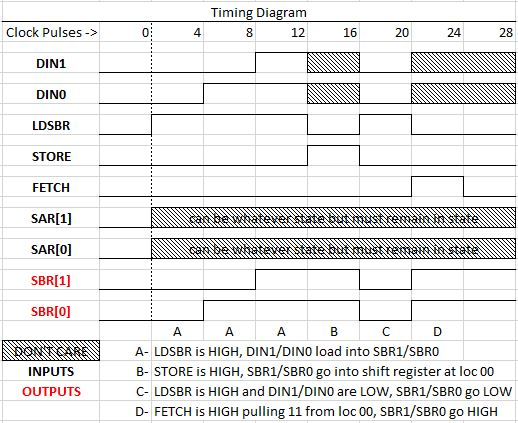
\includegraphics[scale=0.75]{Timing_Diagram.jpg}
	\caption{Timing Diagram for Storage Unit}
	\label{fig:timing-diagram}
\end{figure}

%SECTION : Bibliography
%Insert Bibliography if needed

\end{document}